\chapter{Specifikacija programske potpore}
		
	\section{Funkcionalni zahtjevi}
			
			\textbf{\textit{dio 1. revizije}}\\
			
			\textit{Navesti \textbf{dionike} koji imaju \textbf{interes u ovom sustavu} ili  \textbf{su nositelji odgovornosti}. To su prije svega korisnici, ali i administratori sustava, naručitelji, razvojni tim.}\\
				
			\textit{Navesti \textbf{aktore} koji izravno \textbf{koriste} ili \textbf{komuniciraju sa sustavom}. Oni mogu imati inicijatorsku ulogu, tj. započinju određene procese u sustavu ili samo sudioničku ulogu, tj. obavljaju određeni posao. Za svakog aktora navesti funkcionalne zahtjeve koji se na njega odnose.}\\
			
			
			\noindent \textbf{Dionici:}
			
			\begin{packed_enum}
				
				\item Dionik 1
				\item Dionik 2				
				\item ...
				
			\end{packed_enum}
			
			\noindent \textbf{Aktori i njihovi funkcionalni zahtjevi:}
			
			
			\begin{packed_enum}
				\item  \underbar{Aktor 1 (inicijator) može:}
				
				\begin{packed_enum}
					
					\item funkcionalnost 1
					\item funkcionalnost 2
					\begin{packed_enum}
						
						\item  podfunkcionalnost 1 
						\item  podfunkcionalnost 2
				
					\end{packed_enum}
					\item  funkcionalnost 3
					
				\end{packed_enum}
			
				\item  \underbar{Aktor 2 (sudionik) može:}
				
				\begin{packed_enum}
					
					\item funkcionalnost 1
					\item funkcionalnost 2
					
				\end{packed_enum}
			\end{packed_enum}
			
			\eject 
			
			
				
			\subsection{Obrasci uporabe}
				
				\textbf{\textit{dio 1. revizije}}
				
				\subsubsection{Opis obrazaca uporabe}
					\textit{Funkcionalne zahtjeve razraditi u obliku obrazaca uporabe. Svaki obrazac je potrebno razraditi prema donjem predlošku. Ukoliko u nekom koraku može doći do odstupanja, potrebno je to odstupanje opisati i po mogućnosti ponuditi rješenje kojim bi se tijek obrasca vratio na osnovni tijek.}\\
					

					\noindent \underbar{\textbf{UC$<$broj obrasca$>$ - Brisanje rječnika}}
					\begin{packed_item}
	
						\item \textbf{Glavni sudionik:} Admininistrator riječi
						\item  \textbf{Cilj:} Brisanje rječnika iz sustava
						\item  \textbf{Sudionici:} Baza podataka
						\item  \textbf{Preduvjet:} UC Pregledavanje i odabir rječnika
						\item  \textbf{Opis osnovnog tijeka:}
						
						\item[] \begin{packed_enum}
	
							\item Administrator potvrđuje brisanje rječnika $($UC Potvrda brisanja elementa$)$
							\item Sustav iz baze briše odabrani rječnik
						\end{packed_enum}
					
					\end{packed_item}

					\noindent \underbar{\textbf{UC$<$broj obrasca$>$ - Stvaranje administratora riječi}}
					\begin{packed_item}
	
						\item \textbf{Glavni sudionik:} korijenski administrator
						\item  \textbf{Cilj:} Stvaranje admina riječi
						\item  \textbf{Sudionici:} Baza podataka
						\item  \textbf{Preduvjet:} Prijava korijenskog administratora u sustav $($UC Prijava u sustav$)$
						\item  \textbf{Opis osnovnog tijeka:}
						
						\item[] \begin{packed_enum}
	
							\item Korijenski administrator $($nadalje kAdmin$)$ odabire opciju ”stvori admina riječi”
							\item kAdmin dolazi na stranicu u kojoj mora upisati email adresu i lozinku novog admina riječi $($nadalje rAdmin$)$
							\item kAdmin potvrđuje stvaranje novog rAdmina
							\item Podaci se spremaju u bazu podataka
						\end{packed_enum}
						
						\item  \textbf{Opis mogućih odstupanja:}
						
						\item[] \begin{packed_item}
	
							\item[2.a] kAdmin može upisati email adresu već postojećeg rAdmina
							\item[] \begin{packed_enum}
								
								\item Sustav ga upozorava da vec postoji rAdmin s upisanom email adresom							
							\end{packed_enum}

							\item[2.b] kAdmin unosi email korisnika
							\item[] \begin{packed_enum}
								
								\item Sustav ga upozorava da korisnička adresa ne može bit iskorištena pri stvaranju rAdmina								
							\end{packed_enum}
							
						\end{packed_item}
					\end{packed_item}

					\noindent \underbar{\textbf{UC$<$broj obrasca$>$ - Brisanje administratora riječi}}
					\begin{packed_item}
	
						\item \textbf{Glavni sudionik: }korijenski administrator
						\item  \textbf{Cilj:} Uklanjanje Admina riječi iz sustava
						\item  \textbf{Sudionici:} Baza podataka
						\item  \textbf{Preduvjet:} Prijavljen kAdmin u sustav $($UC Prijava u sustav$)$, postojanje
						rAdmina kojeg se želi izbrisati
						\item  \textbf{Opis osnovnog tijeka:}
						
						\item[] \begin{packed_enum}
	
							\item kAdmin odabire opciju ”pregled rAdmina” i prikazuje mu se popis rAdmina
							\item kAdmin za specifičnog rAdmina odabire opcije ”obriši rAdmina”
							\item Odabirom te opcije mu se nudi prozorčić za potvrdu $($nastavak UC Potvrda brisanja elementa$)$
						\end{packed_enum}
						
					\end{packed_item}

					\noindent \underbar{\textbf{UC$<$broj obrasca$>$ - Registracija učenika}}
					\begin{packed_item}
	
						\item \textbf{Glavni sudionik:} Učenik
						\item  \textbf{Cilj:} Stvaranje učeničkog računa
						\item  \textbf{Sudionici:} Baza podataka
						\item  \textbf{Preduvjet:} Učenik nije registriran niti prijavljen u sustav
						\item  \textbf{Opis osnovnog tijeka:}
						
						\item[] \begin{packed_enum}
	
							\item Učenik odabire opciju ”Registracija”
							\item Učenik unosi ime, prezime, e-mail i potvrđuje prijavu
							\item Učenik se prijavljuje u sustav s generiranom lozinkom (UC Prijava u sustav)							
							\item Sustav učeniku prikazuje obrazac za promjenu inicijalne lozinke (nastavak UC Promjena inicijalne lozinke)
						\end{packed_enum}
						
						\item  \textbf{Opis mogućih odstupanja:}
						
						\item[] \begin{packed_item}
	
							\item[2.a]Učenik se pokušava registrirati e-mail adresom na koju je već prijavljen račun
							\item[] \begin{packed_enum}
								
								\item Sustav upozorava korisnika i onemogućuje mu registraciju							
							\end{packed_enum}

							\item[2.b] Učenik se pokušava registrirati nepostojećom e-mail adresom
							\item[] \begin{packed_enum}
								
								\item Sustav upozorava korisnika i onemogućuje mu registraciju 								
							\end{packed_enum}
							
						\end{packed_item}
					\end{packed_item}

					\noindent \underbar{\textbf{UC$<$broj obrasca$>$ - Promjena inicijalne lozinke}}
					\begin{packed_item}
	
						\item \textbf{Glavni sudionik:} Učenik
						\item  \textbf{Cilj:} Stvaranje računa
						\item  \textbf{Sudionici:} Baza podataka
						\item  \textbf{Preduvjet:} UC Registracija učenika
						\item  \textbf{Opis osnovnog tijeka:}
						
						\item[] \begin{packed_enum}
	
							\item Učenik u obrascu dvaput unosi novu lozinku i potvrđuje unos
							\item Ako se lozinke podudaraju nova se lozinka sprema u bazu i označava da
							je inicijalna lozinka promijenjena
							\item Sustav preusmjerava korisnika na zaslon za odabir jezika (UC Pregledavanje i odabir jezika)
						\end{packed_enum}
						
						\item  \textbf{Opis mogućih odstupanja:}
						
						\item[] \begin{packed_item}
	
							\item[1.a]Učenik gasi aplikaciju
							\item[] \begin{packed_enum}
								
								\item Ponovnom prijavom u sustav korisniku je prikazan obrazac za promjenu lozinke						
							\end{packed_enum}

							\item[2.a] Lozinke se ne podudaraju
							\item[] \begin{packed_enum}
								
								\item Sustav upozorava učenika i traži ispravak unosa  								
							\end{packed_enum}
							
						\end{packed_item}
					\end{packed_item}
				
					
					\subsubsection{Dijagrami obrazaca uporabe}
					
					\begin{figure}[H]
						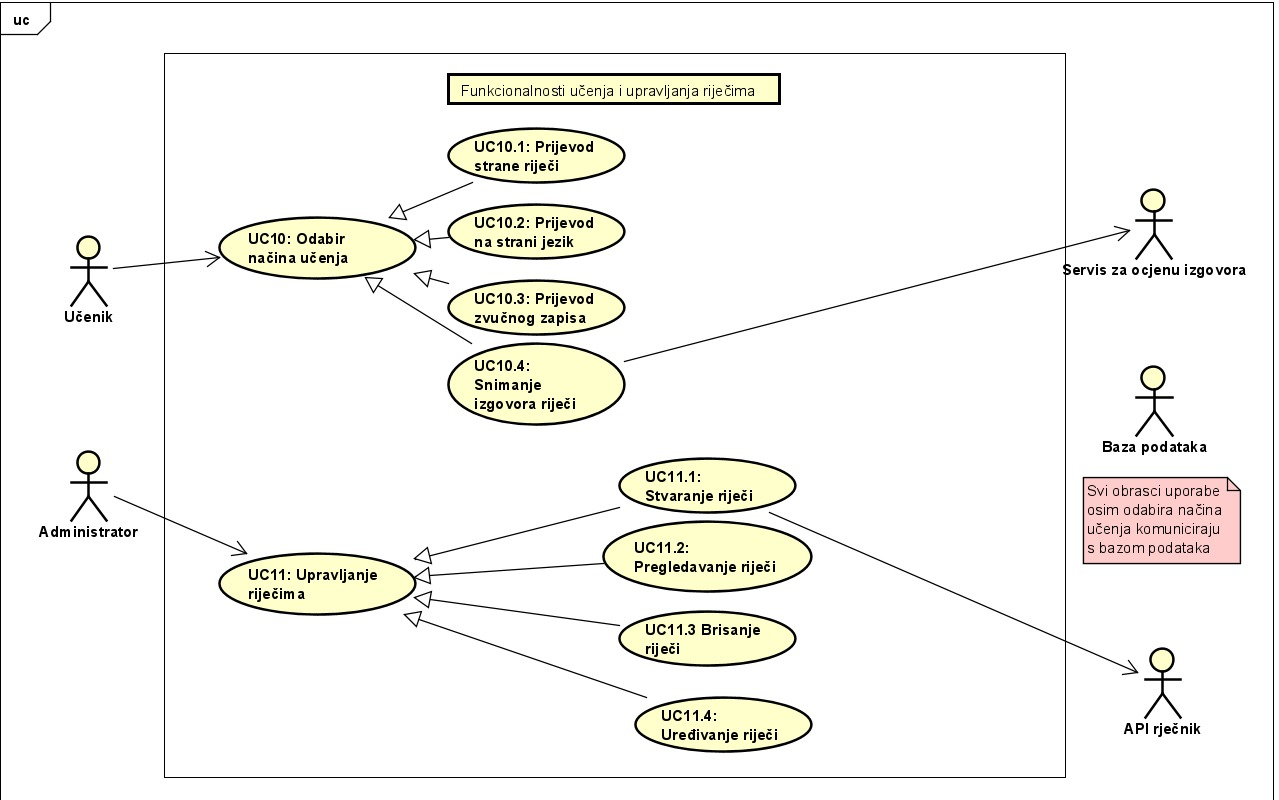
\includegraphics[scale=0.30]{dijagrami/dijagram1.jpg} 
						\centering
						\caption{Funkiconalnosti učenja i upravljanja riječima}
						\label{fig:dijagram1}
					\end{figure}
					
					\begin{figure}[H]
						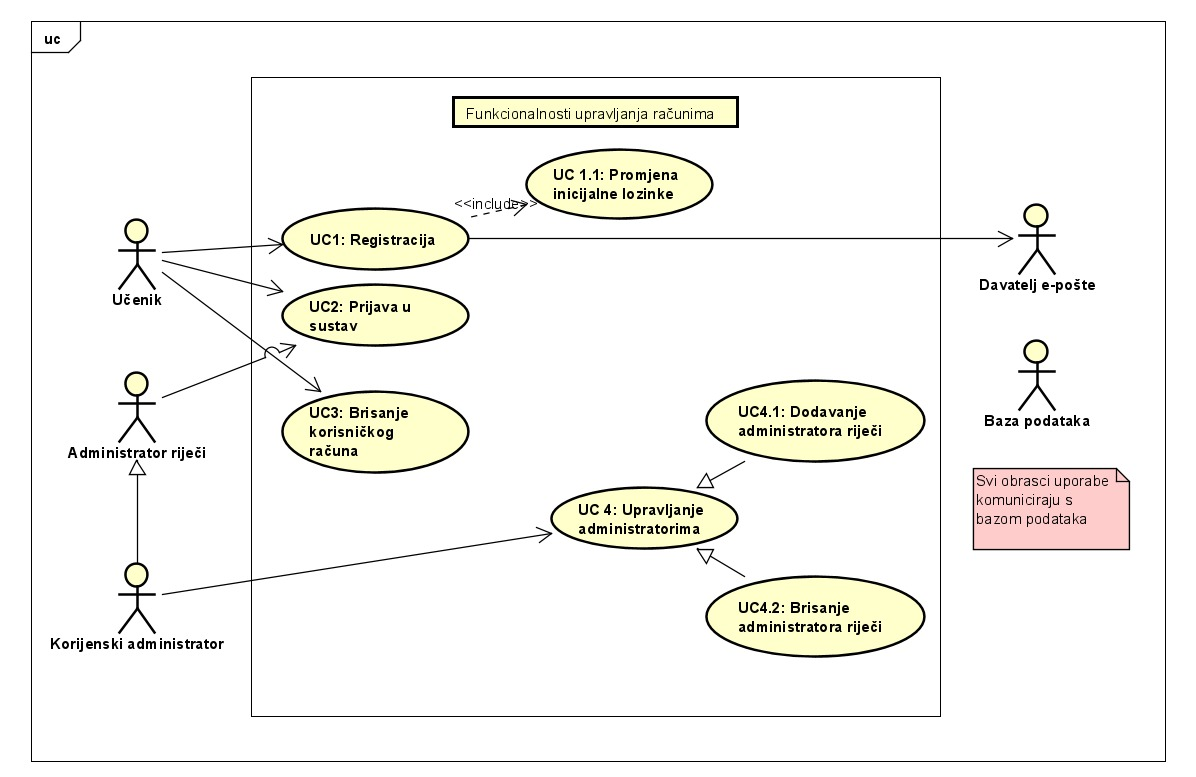
\includegraphics[scale=0.35]{dijagrami/dijagram2.jpg} 
						\centering
						\caption{Funkcionalnosti upravljanja računima}
						\label{fig:dijagram2}
					\end{figure}
					
					\begin{figure}[H]
						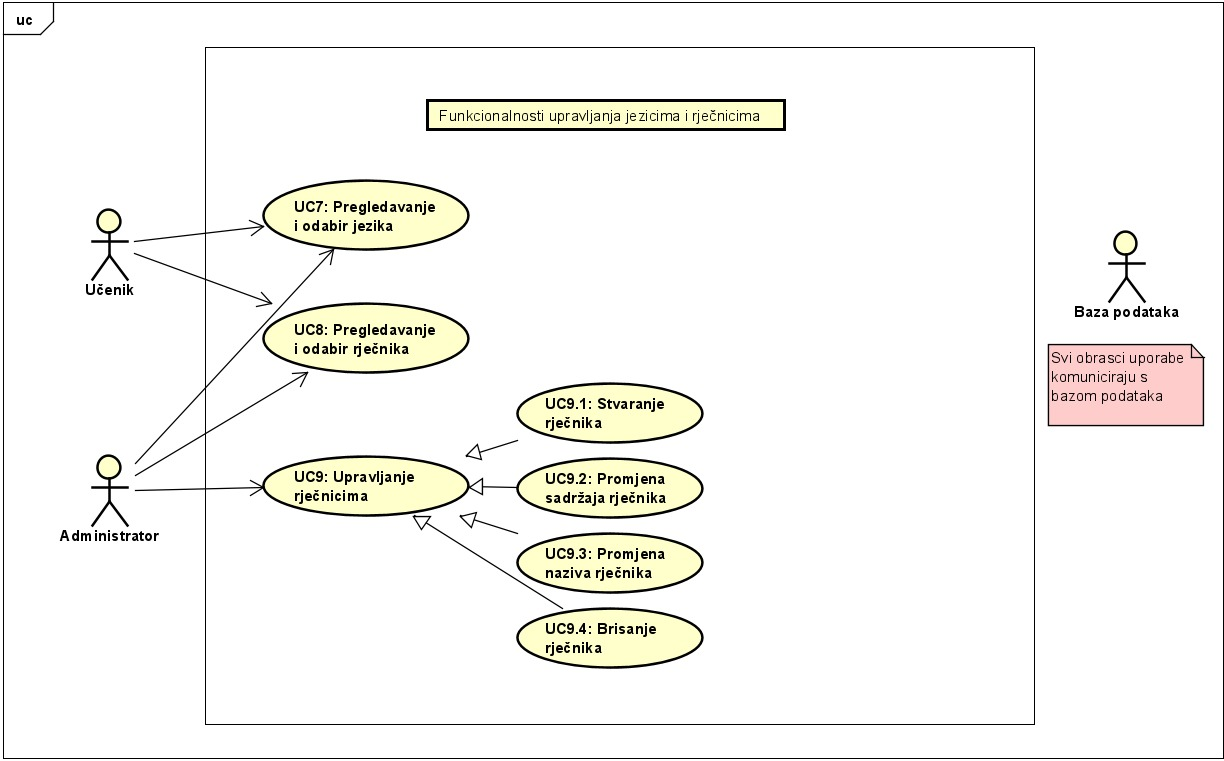
\includegraphics[scale=0.34]{dijagrami/dijagram3.jpg} 
						\centering
						\caption{Funkcionalnosti upravljanja jezicima i rječnicima}
						\label{fig:dijagram3}
					\end{figure}	
				
			\subsection{Sekvencijski dijagrami}
				
				\textbf{\textit{dio 1. revizije}}\\
				
				\textit{Nacrtati sekvencijske dijagrame koji modeliraju najvažnije dijelove sustava (max. 4 dijagrama). Ukoliko postoji nedoumica oko odabira, razjasniti s asistentom. Uz svaki dijagram napisati detaljni opis dijagrama.}
				\eject
	
				\section{Ostali zahtjevi}

				\begin{itemize}
					\item sustav korisniku daje povratnu informaciju o točnosti njegova odgovora
					\item sustav u razumnom vremenu prezentira riječi nakon odabira načina rada
					\item sustav mora imati potporu hrvatskih dijakritičih znakova
					\item sustavu iz javne mreže pristupamo protokolom HTTPS
					\item sustav je dovoljno jednostavan i intuitivan za bilo koju dobnu skupinu korisnika 
					\item za korištenje sustava korisniku je potrebno poznavanje hrvatskog jezika
					\item rječnik mora imati barem 10 riječi
					\item prijevodi rječi moraju biti ispravni
				\end{itemize}
			 
			 
			 
	